\newpage
\chapter{Introduction}
    
    The geometric model of concurrency, studied by Pratt and van Glabbeek \cite{Pratt00Sculptures, pratt91hda, Glabbeek06HDA}, is a useful and general model of non-interleaving concurrency. This model was named \emph{higher-dimensional automata} (HDA) by Pratt \cite{pratt91hda}. In non-interleaving concurrency, we differentiate between concurrent and interleaving executions, using CSS notation \cite{Milner83SCCS}, $a \parallel b \neq a.b + b.a$. Also, more than one event may happen in non-interleaving concurrency. This differentiation is opposite from that of interleaving concurrency where one assumes that $a \parallel b = a.b + b.a$. Since in interleaving concurrency certain actions may be atomic, meaning that these actions are indivisible and instantaneous.
    
    Intuitively, an higher-dimensional automaton is an automaton with nicely incorporated squares, cubes and higher-dimensional cubes, which represent the independence of events. Such a concurrency model is interpreted geometrically, roughly as topological spaces in which paths correspond to executions and two executions are equivalent when the corresponding paths are homotopic. A deformation, where one path can be "\emph{continuously deformed}" into another path, is called a homotopy between the two paths as the two paths are considered homotopic. If two paths are homotopic, then we may consider two paths as being a single path, hence reducing the state space. For our purpose, topological spaces are not exactly the right notion. We need a \emph{directed} variant to incorporate a notion of irreversible time, in other words making it possible to determine the order of an execution.
    
    Higher-dimensional automata are able to also encompass interleaving models and all the other commonly used models of concurrency, such as \emph{transition systems} \cite{winskel95modelsCategory}, \emph{asynchronous transition systems} \cite{Shields85}, \emph{petri nets} \cite{Petri73petrinets}, \emph{event structures} \cite{NielsenPW81eventstructures} and \emph{configuration structures} \cite{GlabbeekP09configStruct}. However, because of the generality of higher-dimensional automata they are challenging to work with. From the work in \cite{Johansen16STstruct} on \emph{ST-structures}, which were introduced as event-based counterpart of higher-dimensional automata, we know that it is not always possible to precisely identify the events in a higher-dimensional automaton. Vaughan Pratt introduced \emph{sculptures} \cite{Pratt00Sculptures} and \emph{Chu spaces} \cite{gupta94phd_Chu, pratt95Chu} as models which retain some good aspects of higher-dimensional automata as well as being easier to work with. Chu spaces have been developed as a response to the event-state duality argued by Pratt \cite{Pratt02eventStateDuality}. However, a study of sculptures has yet to be done.
    
    The subject matter of this thesis is to give a precise definition of sculptures, following the intuition of Pratt, where one can think of the process of modelling a concurrent system using higher-dimensional automata as a \emph{sculpting} process as follows. Take one single higher-dimensional cube, having enough concurrency (that is, enough events) and remove cells until the desired concurrent behaviour is obtained. The model obtained is a sculpture.
    
    We investigate a conjecture posed by Vaughan Pratt at the end of the introduction of \cite{Pratt00Sculptures}. The conjecture is that any higher-dimensional automata can be obtained using the sculpting method. We develop an algorithm to decide whether a higher-dimensional automaton can be sculpted or not, and show several simple examples of \emph{acyclic} higher-dimensional automata which are not sculptures. We believe that this contradicts Pratt's claim cited above.  We also show that there is a close correspondence between sculptures, Chu spaces over 3 \cite{Pratt00Sculptures} and ST-structures.
    
    In Chapter \ref{chap:traditional-models-for-concurrency} and \ref{chap:An introduction to models for true concurrency}, we will review some models of concurrency. We will see the ideas which they contributed to understanding higher-dimensional automata, and also see how they fall short of our intuitions of concurrent behaviour. We will also review some models of concurrency, in Chapter \ref{chap:An introduction to models for true concurrency} and \ref{chap:Relationship with other models of true concurrency}, which contributed ideas to understanding the sculpting method. These are in particular higher-dimensional automata, ST-structures and Chu spaces. Before further delving into the technical details of higher-dimensional automata and sculptures, some general considerations about the nature of concurrency models and their geometric notion might serve as an introduction.
    
    \section{Models of concurrency}
        Models of concurrency which have been studied and used within theoretical computer science depend on mathematics as a foundation in which to describe and reason about the behaviour of concurrency. Whenever a programmer has written a program, they tend to have an idea of how the system should behave. For example, if a programmer writes \emph{if}$(a\ and\ b)\ then\ c$, then the programmer has some idea of how the system would evaluate the statement $a\ and\ b$. This may, or may not, correspond to how the statement is actually evaluated by the system. Nevertheless, the purpose of a mathematical model is to make precise the intuitions, so that the programmer perceives the program to behave as the actual implementation. In concurrency a program behaves unambiguously making mathematical models absolutely necessary. The goal of mathematical models is to provide an understanding of systems and their behaviour in theory, and to contribute to methods of analysis and design in practice.

        Models of concurrency have a concept of states, where a state is a snapshot of a system at a particular moment. These models also have a concept of transitions, which is a way of moving from one state to another. Various models represent these transitions as \emph{actions} and \emph{events}. Transition systems, asynchronous transition systems and higher-dimensional automata, are \emph{action based}, and also state-based, models because any transition can occur repeatedly. Configuration structures, event structures and ST-structures are \emph{event-based} models, where each event can occur at most once during the execution of a process. Intuitively, actions are labels on events, and may occur repeatedly, and events occur only once and are labeled by actions. For example, consider someone sending an email to two different people. We have that the "send" action is repeated, however, these are considered two distinct events since the email is sent to two different recipients.
    
        Event-based models use labelling functions to represent multiple occurrences of an action, so that each event is labeled with an action. In an event-based model there are no loops, that is, after moving out from a state a system can never return to that state. Also, event-based models are able to capture the entire history of a process. The main disadvantage of storing the entire history is that processes which can be represented by small structures in a state-based model may need an infinite structure in the event-based model. Because of the repetitive nature of state-based models, for example, loops in a transition system. However, representing each event explicitly allows event-based models to be formulated as categories. A category is an abstraction of a mathematical concept that provides a way of relating mathematical structures by structure-preserving functions.\footnote{The standard introduction to category theory is the classical book by Mac Lane \cite{CategoryTheory71Mathematician}, which is aimed at mathematicians. For an introduction to category theory in computer science, the book by Pierce \cite{CategoryTheory91ComputerScientist} is aimed at theoretical computer scientist.} Having a history of each occurrence of an action makes the information content of each state very clear, making them close to domain theory and providing them with a schedule-automata duality \cite{NielsenPW81eventstructures, GlabbeekP09configStruct}, also called \emph{event-state duality}. 
   
        Another way to classify models of concurrency is as \emph{interleaving} and \emph{non-interleaving}. Interleaving models have actions which are \emph{atomic} or indivisible, and the parallel execution of two atomic actions is considered equivalent to executing them in either order, that is, satisfying the law: $a \parallel b = ab \cup ba$. Transition systems are examples of interleaving models. Non-interleaving models allow the splitting up of an action into several smaller actions, and the parallel execution of two actions are considered to have no information about the order relation of those actions. This is regarded as different from $ab \cup ba$, which represents the choice between $ab$ and  $ba$. Asynchronous transition systems, event structures, higher dimensional automata, ST-structure and Chu spaces are non-interleaving models.
    
        In Section \ref{sec:traditional-concurrency-summary}, we attempt to provide some intuition on the difference between interleaving and non-interleaving models, which have been shown to interpret the event-state duality differently \cite{pratt91hda, Pratt02eventStateDuality}. In interleaving models, the interpretation of the event-state duality is as shown by Winskel et al. \cite{NielsenPW81eventstructures} and van Glabbeek \cite{GlabbeekP09configStruct}. For non-interleaving models, there is still a need of further investigation of the event-state duality. However, Chu spaces were created as a response to solve the event-state duality \cite{gupta94phd_Chu}. In Section \ref{sec:summary-4-relationship}, we touch upon the event-state duality of the models of concurrency presented in Chapter \ref{chap:An introduction to models for true concurrency}.
    
        Interleaving models assume actions to be instantaneous, such that for some kinds of observations the two processes $a \parallel b$ and $ab \cup ba$ are observably the same \cite{GlabbeekV97splitting}. With this assumption, we are able to have a tractable algebraic theory. On the other hand, the interleaving assumption forces actions to be regarded as atomic. Atomic actions impose a certain abstraction level to be the lowest granularity level \cite{GlabbeekG89refinement, GlabbeekG01refinement, pratt91hda}. For example, a programmer may give details on actions that, at the time, are regarded as atomic. However, at a future release the programmer may discover that the actions have substructures, see \cite[Example 1.1]{GlabbeekG89refinement}. The programmer cannot refine the action since it is atomic. In Section \ref{sec:traditional-concurrency-summary}, we advocate for refinement of actions and provide Pratt's interpretation of refinement \cite{pratt91hda}. Hence, we are interested in non-interleaving models, presented in Chapter \ref{chap:An introduction to models for true concurrency}, that have an algebraic structure. Having an algebraic structure provides a tractable algebraic theory to reason about the behaviour of concurrency mathematically.
   
    \section{Refinement of actions}
        Concurrent systems should have the possibility to be developed incrementally by starting from an abstract specification and gradually obtaining more details. An incremental approach would be able to update existing systems rather than implementing new systems. Naturally, such systems would be considered efficient and reliable. In concurrent systems, the incremental development can be done by refining actions.
        
        Refinement of actions can be considered for both interleaving and non-interleaving models. For interleaving, a refinement is often found in process algebras where an implementation refines a specification by reducing the set of execution traces. The set of execution traces is reduced when the non-determinism of a specification is removed. Non-interleaving models regard refinement to be a refinement of actions, called \emph{action refinement}. Action refinement is the method of developing a system by starting with an abstract specification, and gradually refining its action, by providing more details. Hence, an action can be changed from being instantaneous, as with interleaving, to having structure, or duration.
        
        If we consider the use of action refinement in the programmer example above, then the programmer is able to provide an abstract specification at first release and at future releases give more details to actions. Action refinement will not be presented here, however, for a detailed example consider the example presented by van Glabbeek in \cite[Example 1.1]{GlabbeekG89refinement}.
        
        With non-interleaving models we are able to consider a system at any abstraction level by refining actions. In Section \ref{sec:asynchronous-transition-systems}, we will show that some non-interleaving models are only able to reason about the independence of pairs of events, where we might naturally need to reason about an arbitrary number of independent events. 
   
   
   \section{Geometric models of concurrency}
        Geometric models of concurrency are non-interleaving models with an algebraic structure, which provides an algebraic theory for non-interleaving models. Geometric models are useful and general since they are able to capture the behaviour of other interleaving and non-interleaving models \cite{Goubault18RelationshipsModelsForConcurrency}, such as transition systems and asynchronous transition systems \cite{Fajstrup16DirectedAlgebraicTopologyConcurrency}. Geometric models enable the use of techniques from algebraic topology in order to study concurrent behaviour. Van Glabbeek in \cite{Glabbeek06HDA} considered higher-dimensional cubes as a natural way of interpreting concurrency, which lead to the development of higher-dimensional automata \cite{Glabbeek06HDA, Goubault95PhDThesis, pratt91hda}. Goubault furthered the development of higher-dimensional automata by showing that many of the other models of concurrency, such as event structures, transition systems and asynchronous transition systems, could be interpreted in terms of higher-dimensional automata \cite{Goubault95PhDThesis, Goubault18RelationshipsModelsForConcurrency}. Higher-dimensional automata can be seen as a generalization of other models of concurrency.
        
        ST-structures were introduced by Johansen in \cite{Johansen16STstruct} as the event-based counterpart of higher-dimensional automata. With an event-based model, we are able to make the information content of each state very clear. As shown by Johansen in \cite{Johansen16STstruct}, higher-dimensional automata are highly expressive and capture the main characteristic of interleaving and non-interleaving models. However, higher-dimensional automata cannot precisely identify events, such as the asymmetric conflict shown in \cite[Figure 5]{Johansen16STstruct}. We will attempt to identify events in higher-dimensional automata in Chapter \ref{chap:Relationship with other models of true concurrency}. We will also present Chu spaces since they are considered to be a response to the state-event duality of Pratt \cite{Pratt02eventStateDuality}. With Chu spaces we can reconcile the relationship between ST-structures and higher-dimensional automata, but also introduce sculptures.
        
        In the meanwhile, we provide the following short summary. We will be considering traditional models of concurrency to see the ideas which they contribute to understanding higher-dimensional automata. We are interested in studying models for concurrency that follow the principle of non-interleaving concurrency, but in relation to the state-based model of higher-dimensional automata. In particular, models based on sets of events. With such models, we are able to precisely identify the events making the information content of each state very clear. We focus on identifying events in higher-dimensional automata. Specifically, by transforming Chu spaces \cite{gupta94phd_Chu}, ST-structures \cite{Johansen16STstruct} and sculptures into equivalent higher-dimensional automata. Our goal is to challenge a conjecture posed by Vaughan Pratt in \cite{Pratt00Sculptures}, at the end of the introduction of \cite{Pratt00Sculptures}.
        
        In higher-dimensional automata one can think of the process of modelling a concurrent system using higher-dimensional automaton as a \textit{sculpting} process as follows. Take one single higher-dimensional cube, having enough concurrency, that is, enough events, and remove cells until the desired concurrent behaviour is obtained. This is different than what is usually done in process algebras where a system is built by composing together smaller systems, which in higher-dimensional automata is done by gluing together cubes.
    
        The conjecture is that any higher-dimensional automaton can be obtained using the sculpting method. To answer this we first need to define precisely the sculpting method, following again the intuition of Pratt that sculpting is similar to subalgebras. More intuitions and examples are in Chapter \ref{chap:sculpting-in-concurrency} where we define sculptures.  We develop an algorithm to decide whether an higher-dimensional automaton can be sculpted or not, and show several simple examples of \emph{acyclic} higher-dimensional automata which are not sculptures. We believe that this contradicts Pratt's conjecture. We also identify exactly the class of higher-dimensional automata that are sculptures.
        
        \begin{center}
            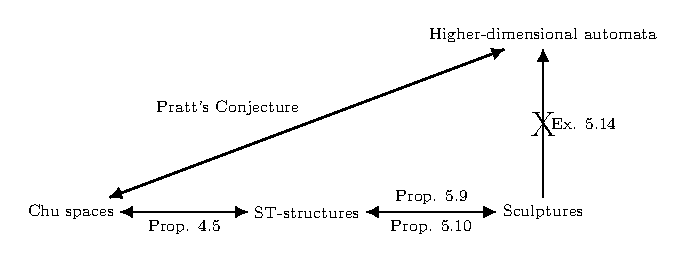
\includegraphics[scale=1]{Figures/4.Relationship-with-other-models-of-concurrency/Chu-spaces-and-ST-structures/argument-diagram.pdf}
        \end{center}
        
        In Proposition \ref{prop:ST-structure-Chu-over-3}, we show the isomorphism between Chu spaces and ST-structures. Furthermore, we provide further proof in Proposition \ref{prop:ST-to-Sculpture} and Proposition \ref{prop:Sculpture-to-ST} that ST-structures and sculptures are isomorphic. Hence, sculptures are also isomorphic to Chu spaces. To strengthen the proofs, we provide examples of higher-dimensional automata which are not sculptures, see Example \ref{exp:hda-broken-box}. We use this example to show the \emph{non-sculpting} theorem.
        